\documentclass[zavrsnirad]{../fer}
% Dodaj opciju upload za generiranje konačne verzije koja se učitava na FERWeb
% Add the option upload to generate the final version which is uploaded to FERWeb

\usepackage{float}
\usepackage{blindtext}
\usepackage{subcaption}
\usepackage{hyperref}
\newtheorem{teorem}{Teorem}

%--- PODACI O RADU / THESIS INFORMATION ----------------------------------------

% Naslov na engleskom jeziku / Title in English
\title{Galjerkin finite element method}

% Naslov na hrvatskom jeziku / Title in Croatian
\naslov{Galjorkinova metoda konačnih elemenata}

% Broj rada / Thesis number
\brojrada{1884}

% Autor / Author
\author{Hrvoje Radoš}

% Mentor 
\mentor{prof. dr. sc. Tomislav Burić}

% Datum rada na engleskom jeziku / Date in English
\date{June, 2025}

% Datum rada na hrvatskom jeziku / Date in Croatian
\datum{lipanj, 2025.}

%-------------------------------------------------------------------------------


\begin{document}


% Naslovnica se automatski generira / Titlepage is automatically generated
\maketitle


%--- ZADATAK / THESIS ASSIGNMENT -----------------------------------------------

% Zadatak se ubacuje iz vanjske datoteke / Thesis assignment is included from external file
% Upiši ime PDF datoteke preuzete s FERWeb-a / Enter the filename of the PDF downloaded from FERWeb
\zadatak{Files/zadatak.pdf}


%--- ZAHVALE / ACKNOWLEDGMENT --------------------------------------------------

\begin{zahvale}
	% Ovdje upišite zahvale / Write in the acknowledgment
Htio bih se zahvaliti svom mentoru,
prof. dr. sc. Tomislavu Buriću, 
na pomoći pri izradi ovog rada,
prof. dr. sc. Dariu Bojancu, koji me prvi upoznao
s temom konačnih elemenata, te mom profesoru iz fizike,
Ivici Marinoviću, koji je imao najznačajniji 
utjecaj na moje matematičke i analitičke sposobnosti,
i samim time dao dosad najveći
doprinos meni osobno tijekom moga obrazovanja.
\end{zahvale}


% Odovud započinje numeriranje stranica / Page numbering starts from here
\mainmatter


% Sadržaj se automatski generira / Table of contents is automatically generated
{\large
\tableofcontents
}

%--- UVOD / INTRODUCTION -------------------------------------------------------
\chapter{Uvod}
\label{pog:uvod}
Diferencijalne jednadžbe su jedan od temeljnih matematičkih
alata koji se koriste za matematičko modeliranje. Njihova
važnost se obično prvo primijeti u fizici gdje se one vrlo
intuitivno pojavljuju u područjima kao što su klasična mehanika,
elektromagnetizam, termodinamika pa i malo manje intuitivno u
područjima kao što su kvantna mehanika. Diferencijalne jednadžbe
imaju veliku uporabu i u područjima izvan fizike.
S njima se mogu modelirati izmjene populacija, širenje zaraza,
oblikovanje raznih genetskih obilježja (uzoraka),
širenje signala u neuronima, procesiranju slika, raznim
modeliranjima tržišta itd.
\bigskip
\\
Diferencijalne jednadžbe uglavnom nije teško tumačiti. Najveći
izazov kod rada s njima je svakako traženje rješenja.
Rješenje ne mora uvijek postojati, ne mora biti jedinstveno,
a ako postoji i jedinstveno je ne mora biti moguće zapisati
ga analitički. Tim problemima se između ostaloga bavi numerička
matematika. Ovaj rad se bavi linearnim parcijalnim diferencijalnim
jednadžbama s konstantnim koeficijentima i rubnim uvjetom odnosno
traženjem njihova rješenja koristeći Galjorkinovu metodu
konačnih elemenata. Cilj rada je pokušati  napraviti
C++ biblioteku koja služi kao efikasan, ali iznad svega
jednostavan alat za rješavanje PDJ-ova. 
% Neki od radova koje ćemo citirati su \cite{6248073,6247753,ghiglia_pritt_phase_unwrapping,hartley2003multiple,4250461,123DCatch}.
\newpage
\subsection{Definicije i primjeri}

Parcijalne diferencijalne jednadžbe su diferencijalne 
jednadžbe koje sadrže derivacije nepoznate funkcije s
obzirom na više varijabli. Označimo s $u$ nepoznatu funkciju
koju želimo odrediti s $d + 1$ nepoznatih varijabli 
$\textbf{x} = (x_1, \dots, x_d)^T$ i $t$. Općenita parcijalna diferencijalna 
jednadžba (PDJ) poprima oblik:
$$\mathcal{P}(u, g) = F(\textbf{x}, t, u,
\frac{\partial u}{\partial t},
\frac{\partial u}{\partial x_1},
\dots,
\frac{\partial u}{\partial x_d},
\dots
\frac{\partial^{p_1 + \dots + p_d + p_t} u} 
{\partial x_1^{p_1}\dots\partial x_d^{p_d} \partial t^{p_t}}
) = 0$$
gdje $g$ predstavlja skup parametara o kojima PDJ ovisi, a 
$p_1, p_2, \dots, p_d, p_t \in \mathbb{N}$. Kažemo da 
je PDJ reda $q$ ako je $q$ maksimalna vrijednost izraza 
$p_1 + p_2 + \dots + p_d + p_t$. 
Ako $\mathcal{P}(u,g)$ ovisi lineano o nepoznanici $u$ 
i o svojim parcijalnim derivacijama, kažemo da je 
PDJ  linearna.
\bigskip
\\ 
Linearne PDJ su jako česte u praksi, stoga ću u nastavku 
navesti nekoliko primjera.\\
\textit{Transportna jednadžba}:
$$\frac{\partial u}{\partial t} + \nabla \cdot (\beta u) = 0$$
$\nabla \cdot v$ označava operator divergencije odnosno 
$\nabla \cdot v = \sum_{i=1}^d \frac{\partial v}{\partial x_i}$
\bigskip 
\\
PDJ kojom ću se u ovom radu većinom
baviti je \textit{jednadžba potencijala} koja
se također može koristiti za opis vertikalnog
pomaka elastične membrane. 
\begin{equation}
  \label{potencijalPDJ}
- \Delta u = - f 
\end{equation}
\\ 
U praksi je od iznimne važnosti i \textit{jednadžba vođenja topline}
\begin{equation}
  \frac{\partial u}{\partial t} - \Delta u = f
\end{equation}
\bigskip 
\\ 
S $\Delta$ označavam Laplaceov operator.
$\Delta u = \sum_{i = 1}^d \frac{\partial^2 u}{\partial x_i ^2}$ 
\bigskip 
\\
\textit{Valna jednadžba}
\begin{equation}
  \frac{\partial ^2 u}{\partial^2 t} - \Delta u = 0
\end{equation}

Iako im u ovom radu nisam posvetio
dovoljno veliku pažnju kakvu 
inače zaslužuju, navodim 
i neke nelinearne PDJ.
Jedna od njih se zove \textit{Burgersova jednadžba}.
$$\frac{\partial u}{\partial t} +
u \frac{\partial u}{\partial x_i}$$
Burgersova jednadžba je korištena u modelima fluida, 
nelinearnoj akustici te čak u modeliranju toka prometa. 
\\
Pred kraj dajem proizvoljnu nelinearnu PDJ. 
$$\Big(\frac{\partial^2 u}{\partial x_1 ^2}\Big)^2 +
\Big(\frac{\partial^2 u}{\partial x_2 ^2}\Big)^2 = f$$

\subsection{Numeričko rješenje}
Općenito nije moguće pronaći rješenje od $\mathcal{P}(u,g)$ 
u eksplicitnom obliku. Neke stardardne metode kao što 
su separacija varijabli su veoma ograničene po tom pitanju.
Čak kada je poznato opće rješenje ne mora biti moguće pronaći 
partikularno, što dovodi do nužnosti postavljanja takozvanih 
rubnih uvjeta na  ove jednadžbe. Rubni uvjeti su matematički izrazi 
koji zahtijevaju da se nepoznata funkcija specifično ponaša
na rubu njezine domene.
\bigskip
\\ 
Mogućnost odabira proizvoljnih rubnih uvjeta značajno 
podiže složenost ovog problema. Iz perspektive matematičke 
teorije, analiza PDJ-ova je uglavnom ograničena na  
postojanje, jedinstvenost i regularnost rješenja, no 
nedostaju moćni alati za njihovo rješavanje. 
\bigskip
\\ 
Iz gornje rasprave slijedi da je bitno imati 
razvijene numeričke metode za rješavanje PDJ-ova koje 
ne rješavaju danu parcijalnu jednadžbu, nego daju dovoljno 
dobru aproksimaciju njezina rješenja. 
\newpage 

\subsection{Klasifikacija parcijalnih diferencijalnih jednadžbi}
Parcijalne diferencijalne jednadžbe se mogu svrstati u 
tri različite kategorije \textit{eliptičke},
\textit{paraboličke} i \textit{hiperboličke}.
\\
Radi konciznosti ograničit ću ovo podpoglavlje na linearne PDJ-ove s 
konstantnim koeficijentima oblika:
$$
A\frac{\partial^2 u}{\partial x_1^2}
+ B \frac{\partial^2 u}{\partial x_1 \partial x_2}
+ C \frac{\partial^2 u}{\partial x_2^2}
+ D \frac{\partial u}{\partial x}
+ E \frac{\partial u}{\partial y}
+ F u = G
$$
Gdje $A,B,C,D,E,F,G \in \mathbb{R}$.
Klasifikacija se radi na temelju vrijednosti $\Delta = B^2 - 4AC$
\begin{center}
  Ako $\Delta < 0$, jednadžba je eliptička\\ 
  Ako $\Delta = 0$, jednadžba je parabolička\\ 
  Ako $\Delta > 0$, jednadžba je hiperbolička 
\end{center}
Za kasnije je bitno uočiti da je jednadžba
potencijala \ref{potencijalPDJ}
eliptička. 

%-------------------------------------------------------------------------------
\chapter{Glavni dio}
\label{pog:glavni_dio}
Galjorkinova metoda konačnih elemenata je složen proces
koji se sastoji od više dijelova. Na početku ovog 
poglavlja nudim kratki opis kako ovaj proces izgleda, a
u narednim poglavljima ulazim u detalje.
\bigskip
\\ 
Jednadžba koju rješavam na domeni $\Omega \subset \mathbb{R}^2$ je:

\begin{equation}
\label{PDJ}
C_0 \frac{\partial^2 u}{\partial x^2}
+ C_1 \frac{\partial^2 u}{\partial x \partial y}
+ C_2 \frac{\partial^2 u}{\partial y^2}
+ C_3 \frac{\partial u}{\partial x}
+ C_4 \frac{\partial u}{\partial y}
+ C_5 u = f(x,y)
\quad u \in C^2(\Omega)
\end{equation}

Ključna ideja ove metode je particioniranje domene na
što sitnije odnosno finije dijelove koje nazivamo elementima.
Takvu particiju nazivamo mesh. S meshom potom definiramo
bazne funkcije koje čine bazu s kojom ćemo interpolirati
rješenje koje tražimo. Dodatnim raspisivanjem ćemo dobiti
linearni sustav čijim rješavanjem dobivamo naše traženo
rješenje.
\bigskip
\\ 
\label{uvjetNaf}
Postoji par napomena koje valja primijetiti. Ako obratimo
pažnju na jednadžbu \eqref{PDJ}, možemo primijetiti da smo
se ograničili na rješenja iz prostora $C^2(D)$ dodatnom analizom
možemo zaključiti i da funkcija $f$ mora biti neprekinuta.
Ovo se na prvu iz perspektive primjene ne čini kao velika 
restrikcija jer nekako očekujemo da će fizikalne veličine u 
stvarnom životu uvijek biti neprekinute, ali ne samo da to nije
uvijek slučaj to jako često nije slučaj. Kao primjer navodim 
primjer djelovanja sile (npr. ovješen uteg) na nit. Za modeliranje
ovakvog sustava je potrebno opisati djelovanje te sile duž
cijelu nit, ali takav opis bi zahtijevao uporabu Diracove delta 
funkcije koja nikako nije neprekinuta, štoviše ona nije
ni funkcija nego distribucija.

\begin{figure}[htb]
	\centering
	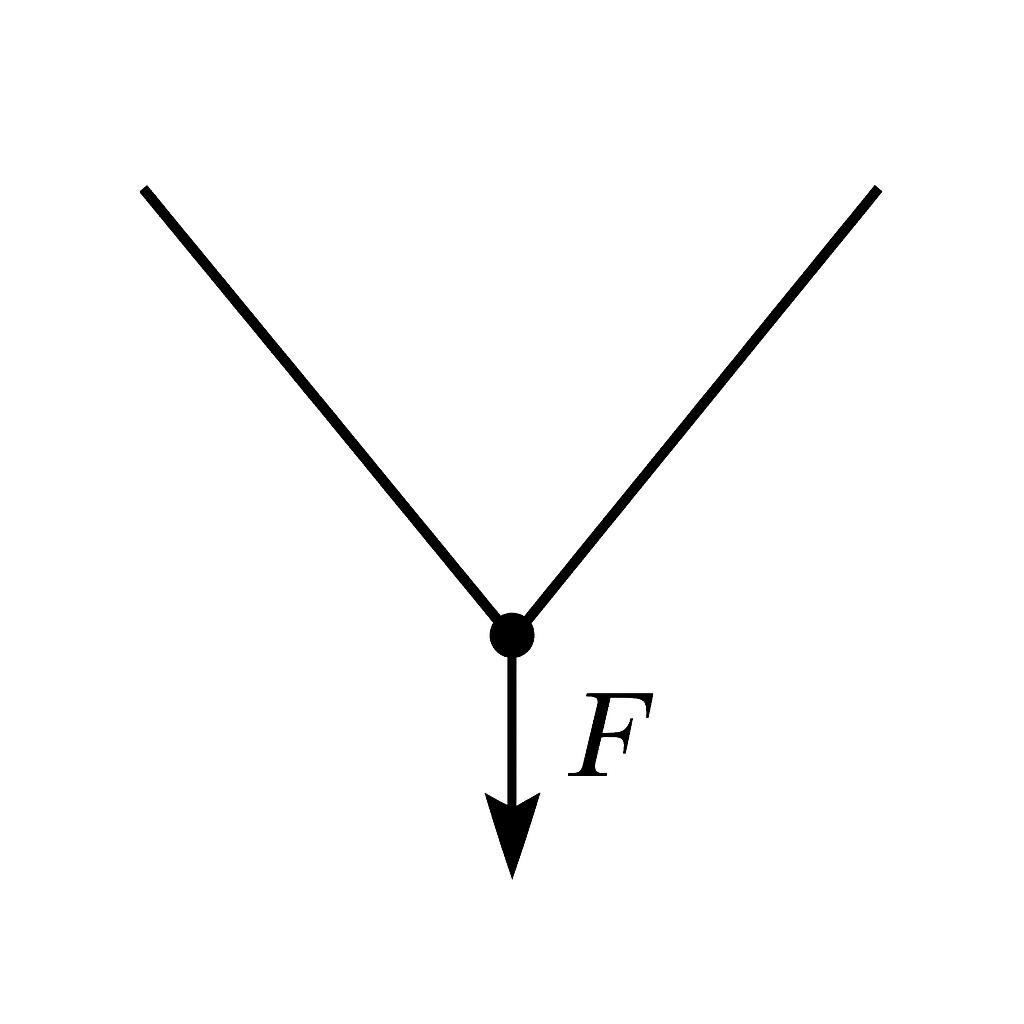
\includegraphics[width=0.38\linewidth]{Figures/nit.png}
	\caption{Djelovanje točkaste sile na nit}
	\label{nit}
\end{figure}

\section{Mesh}
\label{mesh}
Mesh je particija domene na sitne dijelove s kojima ju
možemo aproksimirati. U ovoj implementaciji ti dijelovi 
će biti trokuti (jer radimo s 2D domenom), pa ću proces
stvaranja mesha često zvati i triangulacija. Ti sitni 
dijelovi koji sačinjavaju mesh se zovu elementi. 
Odavde i naziv "metoda konačnih elemenata". Točke koje
čine jedan element (npr. vrhovi trokuta koji predstavlja
jedan elemente) ću u ovom radu zvati čvorovima.

\begin{figure}[htbp]
  \centering
  \begin{subfigure}[b]{0.45\linewidth}
    \centering
    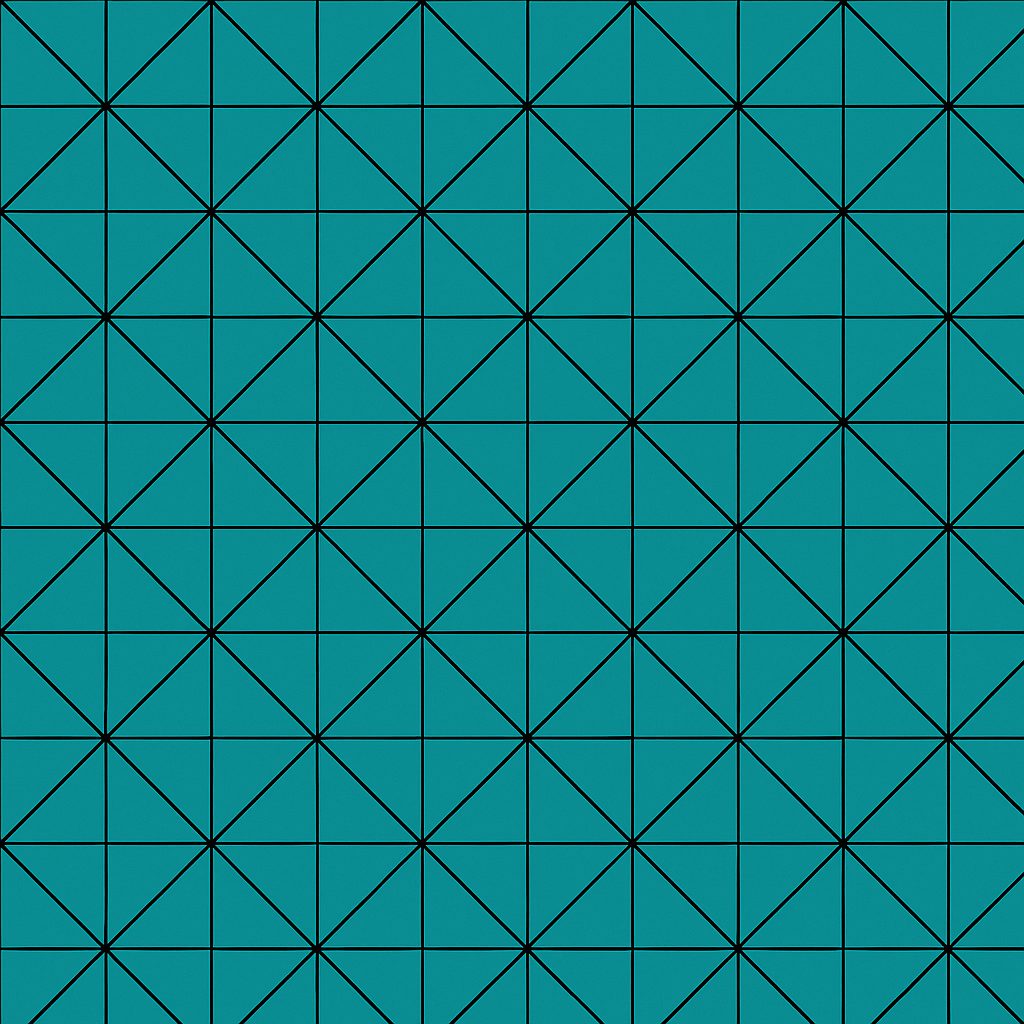
\includegraphics[width=\linewidth]{Figures/2Dmesh.png}
    \caption{Primjer 2D mesha pravokutnika}
    \label{rectMesh}
  \end{subfigure}
  \hfill
  \begin{subfigure}[b]{0.45\linewidth}
    \centering
    
\includegraphics[width=\linewidth]{Figures/apple.png}
    \caption{Složeni 3D mesh jabuke.\href{https://pixabay.com/vectors/apple-fruit-green-apple-nature-1590131/}{Slika}}
    \label{jabuka}
  \end{subfigure}
  \caption{Primjeri mesheva}
  \label{meshevi}
\end{figure}

Bitno je napomenuti kako izbor mesha ne smije biti 
proizvoljan. Postoje kvalitetni i manje kvalitetni 
meshevi. U literaturi ne postoji nekakav jedinstveni 
kriterij koji mesh mora zadovoljavati, tako da 
je generiranje mesha u primijeni uvijek heuristički 
algoritam.
Očito je za zaključiti da bi mesh trebao pravilno popločavati
domenu tj. da ne bi smio sadržavati rupe koje u potpunosti
pripadaju domeni i da bi trebao što bolje aproksimirati domenu
kako su elementi manji odnosno kako je mesh finiji.
\bigskip
\\ 
Svakako valja napomenuti da ne želimo imati previše izdužene
elemente, stoga uvodimo sljedeći kriterij.
$$\frac{h_k}{\rho_k} \leq C$$
Gdje je $h_k$ duljina najdulje stranice trokuta, a 
$\rho$ je promjer upisane kružnice promatranog 
elementa. Razlog zašto ovakav kriterij smanjuje 
izduženost jednog elementa se lako vidi na sljedećoj
slici.
\begin{figure}[htb]
	\centering
	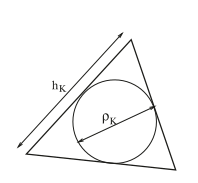
\includegraphics[width=0.38\linewidth]{Figures/element.png}
	\caption{najdulja stranica trokuta $h_k$ i promjer
  upisane kružnice $\rho_k$. Slika je preuzeta iz \cite{Quarteroni}}
\end{figure}

\newpage
\subsection{Bazne funkcije}

Nakon uspješno generiranog mesha potrebno je definirati
bazne funkcije. Bazne fukcije ćemo definirati tako da
na svakom elementu definiramo polinom prvog stupnja koji
iznosi $1$ iznad jednog vrha, a $0$ iznad ostalih \ref{baznaFja}
\begin{figure}[htb]
	\centering
	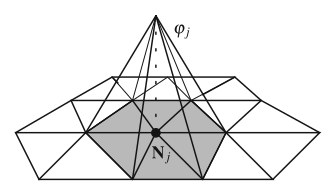
\includegraphics[width=0.5\linewidth]{Figures/baznaFja.png}
  \caption{Bazna fukcija za neki čvor $j$. Slika je preuzeta iz \cite{Quarteroni}}
	\label{baznaFja}
\end{figure}
Ovo ćemo napraviti za svaki čvor. 
\bigskip
\\ 
Kada budemo radili račun kao što su numerička integracija i 
slično nad elementima bit će od velike koristi transformirati
koordinate tako da element koji trenutačno računamo postane 
oblika pravokutnog trokuta s vrhovima u $(0,0)$,$(1,0)$,$(0,1)$. 
Takav trokut se u literaturi uobičajeno zove referentni element.
Neka su $(X_0, Y_0)$,$(X_1, Y_1)$,$(X_2, Y_2)$ vrhovi elementa
kojeg želimo preslikati. Supstitucija $(x, y) \rightarrow (\hat x, \hat y)$
je dana s:
\begin{align}
  x = (X_1 - X_0)\hat x + (X_2 - X_0)\hat y + X_0 \\ 
  y = (Y_1 - Y_0)\hat x +(Y_2 - Y_0) \hat y + Y_0
\end{align}
Potrebno je odrediti kako točno glase bazne funkcije nad 
referentnim elementom.
Indeksirajmo čvor $(0,0)$ s $0$, čvor $(1,0)$ s $1$a i 
čvor $(0, 1)$ s $2$.
Imamo:
\begin{align}
\varphi_0(x,y) = 1 - x - y\\
\varphi_1(x,y) = x\\
\varphi_2(x,y) = y
\end{align}
\newpage
\section{Slaba formulacija problema}
\label{slabaFormulacija}
Radi daljnje analize potrebno je navesti jedan bitan 
teorem.
\\ 
\begin{teorem}[Pravilo za divergenciju produkta]
\label{tm1}
Neka je $\Omega \subset \mathbb{R}^n$ omeđen otvoreni
skup s komadno glatkom granicom $\Gamma = \partial \Omega$,
te neka su $u : \Omega \to \mathbb{R}$ i $\mathbf{V} : \Omega \to \mathbb{R}^n$ 
dovoljne regularnosti odnosno $\partial \Omega$ je
Lipschitz neprekinuta, a $u,v \in H^1(\Omega)$
. Tada vrijedi:
\[
\int_{\Gamma} u \mathbf{V} \cdot \hat{\mathbf{n}} \, d\Gamma = 
\int_{\Omega} u \, \nabla \cdot \mathbf{V} \, d\Omega + 
\int_{\Omega} \nabla u \cdot \mathbf{V} \, d\Omega.
\]
\end{teorem}
\textbf{Napomena:} $H^1(\Omega)$ označava Soboljev prostor.
\bigskip
\\ 
Vratimo se sada na \ref{PDJ}.
Cilj nam je dobiti njezinu takozvanu slabu formulaciju.
Prvo ćemo reformulirati PDJ. Primijetimo da vrijedi:
$$\nabla \cdot (M \nabla u) = 
  C_0 \frac{\partial^2 u}{\partial x^2}
	+ C_1 \frac{\partial^2 u}{\partial x \partial y}
	+ C_2 \frac{\partial^2 u}{\partial y^2}
$$
Gdje:
$$M = 
\begin{pmatrix}
  C_0 & C_1 \\ 
  0 & C_2
\end{pmatrix}
 $$
 Također vrijedi:
 $$ \nabla u \cdot a =
 C_3 \frac{\partial u}{\partial x}
	+ C_4 \frac{\partial u}{\partial y} $$

Gdje:
$$a = 
\begin{pmatrix}
  C_3\\ 
  C_4
\end{pmatrix}
$$
Uvrštavanjem se dobije sljedeća jednadžba:
\begin{equation}
  \label{vektorVerzija}
\nabla \cdot (M \nabla u)  + \nabla u \cdot a + C_5u = f(x,y)
\end{equation}
Do tkz. slabe formulacije dolazimo tako da obje strane \ref{vektorVerzija} 
pomnožimo
s baznom funkcijom $\varphi_i$, integriramo po $\Omega$
i onda primijenimo  \ref{tm1}.\\ 
Imamo:
\begin{equation}
  \int_{\Omega}\nabla \cdot (M \nabla u) \varphi_i \, d\Omega  + 
  \int_{\Omega} \nabla u \cdot a\varphi_i \, d\Omega  + C_5\int_{\Omega}u\varphi_i\,d\Omega  =
  \int_{\Omega}f(x,y)\varphi_i \, d\Omega 
\end{equation}
Primjenom teorema \ref{tm1} 
dobije se:
\begin{equation}
  \label{kobasica}
  \int_{\partial \Omega}(M \nabla u) \varphi_i \, d\Gamma  - 
  \int_{\Omega}(M \nabla u) \cdot \nabla \varphi_i \, d\Omega  + 
  \int_{\Omega} \nabla u \cdot a\varphi_i \, d\Omega  + C_5\int_{\Omega}u\varphi_i\,d\Omega  =
  \int_{\Omega}f(x,y)\varphi_i \, d\Omega 
\end{equation}
S obzirom na to da su funkcije $\varphi_i$ po definiciji
na rubu jednake $0$, jednadžba 
\ref{kobasica} se 
svede na:
\begin{equation}
  \label{slabaFor}
  -\int_{\Omega}(M \nabla u) \cdot \nabla \varphi_i \, d\Omega  + 
  \int_{\Omega} \nabla u \cdot a\varphi_i \, d\Omega  + C_5\int_{\Omega}u\varphi_i\,d\Omega  =
  \int_{\Omega}f(x,y)\varphi_i \, d\Omega 
\end{equation}
Primijetimo kako u ovakvom obliku funkcija $f(x,y)$ 
na sebi ima puno slabije restrikcije (Sjetimo se \ref{uvjetNaf}).
Odavde ujedno i naziv "slaba formulacija". Primijetimo također 
da je ovakva formulacija ekvivalentna jakoj formulaciji 
kada bismo derivacije u jakoj formulaciji shvatili kao 
derivacije distribucija.
\bigskip
\\
Sada interpolacijom nepoznate funkcije $u$:
$$u = \sum_{j=0}^N \alpha_j \varphi_j$$
dobivamo sustav:
\begin{equation}
\label{linSustav}
A x = b
\end{equation}
Gdje:
\begin{equation}
\label{elMat}
(A)_{i,j} = \int_{\Omega} (M\nabla \varphi_j) \cdot \nabla \varphi_i \, d\Omega + 
\int_{\Omega} (\nabla \varphi_j \cdot a) \varphi_i \, d\Omega +
C_5 \int_{\Omega} \varphi_j \varphi_i \, d\Omega
\end{equation}
$$b_i = \int_{\Omega} f(x,y) \varphi_i \, d \Omega$$

Naime ovaj postupak vrijedi samo s Dirichletovim
rubnim uvjetima. Neka su čvorovi mesha na rubu indeksirani
od $N+1$ do $N_b$.
Kada bi se rješenje na rubu ponašalo kao
$R(x,y)$ gdje $R(x,y) = \sum_{j=N + 1}^{N_b} g_j \varphi_j$,
onda bismo morali napraviti sljedeću
supstituciju:
$$u = \overset{\circ}u + R$$
Sustav \ref{linSustav}
onda postaje:
$$Ax = b - r$$
gdje je:
$$r_i = - \int_{\Omega}(M\nabla R) \nabla \varphi_i \, d \Omega +
\int_{\Omega}(\nabla R \cdot a) \varphi_i \, d \Omega +
C_5 \int_{\Omega} R \varphi_i\, d\Omega
$$
Time smo problem rješavanja PDJ sveli na problem
rješavanja linearnog sustava.
%eventualno možeš pričati o proširenjima za vrijeme
\section{Postojanje rješenja}
\label{postojanje}
%Lax Milgram
Iako se možda na prvi pogled čini da smo gotovi, potrebno 
je vidjeti da rješenje uopće postoji, stoga uvodim 
Lax-Milgramov teorem.
\begin{teorem}
  \label{laxMil}
Neka je $ V $ Hilbertov prostor i neka je $ a: V \times V \rightarrow \mathbb{R} $ bilinearna forma koja zadovoljava:
\begin{itemize}
    \item \textbf{Kontinuitet:} postoji konstanta $ C > 0 $ takva da
    $$
    |a(u, v)| \leq C \|u\|_V \|v\|_V \quad \text{za sve } u, v \in V.
    $$
    
    \item \textbf{Koercitivnost (eliptičnost):} postoji konstanta $ \alpha > 0 $ takva da
    $$
    a(v, v) \geq \alpha \|v\|_V^2 \quad \text{za sve } v \in V.
    $$
\end{itemize}

Tada za svaki linearni funkcional $ f \in V' $ postoji jedinstveno $ u \in V $ takvo da:
$$
a(u, v) = f(v) \quad \text{za sve } v \in V.
$$
\end{teorem}
Lako se vidi da se naš sustav \ref{linSustav} 
može svesti na problem s linearnim funkcionalima iz
\ref{laxMil}. Iz toga se lako zaključuje da
postojanje rješenja možemo garantirati samo za ispravan mesh
(to bi trebala garantirati implementacija) i za eliptičke PDJ što se lako provjeri programski.

\newpage
\section{Implementacijski detalji}
\label{implementacijaOpis}
Sada kada je jasna matematička pozadina 
Galjorkinove metode konačnih elemenata, potrebno je 
obratiti pažnju na implementaciju i implementacijske detalje.
S obzirom na to da je implementacija izvedena u C++-u postoji
dosta različitih optimizacija koje se mogu implementirati,
stoga ih navodim u ovom poglavlju.

\subsection{Generiranje mesha}

S obzirom na to da
je jednostavnost korištenja ključno svojstvo ove implementacije 
odlučio sam se za sljedeći način unosa mesha u računalo.
\bigskip
\\ 
\textbf{Korisnik definira funkciju koja prima koordinate, a
vraća vrijednost "true" ako je točka unutar domene ili
"false" ako je točka izvan domene}
\bigskip
\\ 
Time smo implicitno definirali domenu nepoznate funkcije.
Ovakav pristup omogućava da se domena definira na sličan 
način kako bi to inače radili na papiru iz čega
proizlazi jednostavnost korištenja.
Druge C++ biblioteke za unos mesha uglavnom koriste .msh datoteke.
Ovakav pristup je dobar za komplicirane domene koje se ne mogu
lako definirati s implicitnim funkcijama, ali je presložen za neke
jednostavnije primjene. Valja napomenuti da neke biblioteke 
daju mogućnost da se domena definira preko ključnih riječi kao 
što su "circle" ili "rectangle". U usporedbi s tim rješenjima 
moj pristup daje veću fleksibilnost.
\bigskip
\\ 
Jednostavan način korištenja povlači i težinu implementacije.
Naime, kvalitetan mesh može značajno smanjiti numeričku grešku
rješenja. Naravno greška se uvijek može smanjiti tako da 
učinimo mesh finijim, ali to ne možemo raditi u nedogled.
Ova implementacija mesh generira na poprilično jednostavan način.
Za ulaz ona traži pravokutnik koji omeđuje domenu nad kojom
rješavamo PDJ. Taj pravokutnik se potom triangulira i za mesh
se uzimaju samo elementi čija su sva tri vrha unutar domene.
Ovakav pristup daje nekvalitetan mesh na rubu. Istraživajući
bolje pristupe generiranju mesha otkrio sam razne knjige koje
se bave ovom problematikom. Došao sam do zaključka da 
je ovaj problem previše složen za ovaj rad i stoga smatram da
je za sada bitno napraviti implementaciju koja se može naknadno lako 
nadograditi.
\\
Iako jednostavan pristup ovom problemu funkcionira
mislim da je bitno naglasiti gdje ova implementacija ima
mjesta za napredak u smislu kvalitete mesha, pa ćemo tako 
u nastavku vidjeti kako loš mesh na rubu može uzrokovati 
puno veća odstupanja rješenja od mojih prvotno očekivanih.

\subsection{CSR reprezentacija matrice}
Matrica $A$ u \ref{linSustav} 
često sadrži puno nul elemenata. To se vrlo lako može 
vidjeti iz načina na koji se ona računa. Naime, $(A)_{i,j}$ 
neće biti jednak $0$ samo kada su odgovarajući čvorovi 
mesha ($i$ i $j$) susjedni i ako vrijedi $i = j$.
S obzirom na to da je 
zbog veće preciznosti poželjno da
matrice sustava budu što veće,
uvodi se CSR (eng. compact sparse row)
reprezentacija matrice. Ovaj pojam se može lako objasniti na
sljedećem primjeru.
$$M = \begin{pmatrix}
  a & 0 & f & 0 & g\\ 
  0 & b & k & m & 0\\ 
  h & l & c & 0 & r\\ 
  0 & n & 0 & d & p\\ 
  i & 0 & s & q & e
\end{pmatrix}$$
Na slici \ref{CSR} 
se vidi matrica $M$ zapisana preko CSR. Vidimo da se
ova struktura podataka sastoji od 3 vektora. 
Vektori $A$ i $C$ su jednake veličine kao broj ne nul 
elemenata, a svaki element $R$ odgovara jednom retku.
Matrica $A$ se stvara tako da čitajući redak po redak
s lijeva na desno umećemo elemente matrice $M$ koji 
nisu jednaki $0$. Vrijednost $C_i$ odgovara brojčanoj
vrijednosti stupca u kojem se element $A_i$ nalazi 
a element $R_i$ govori od kojeg indeksa kreće $i-ti$
redak matrice $M$ u vektoru $C$ odnosno $A$. 
\\ 
\bigskip
Dohvat elementa $i,j$ ovakve matrice se vrlo lako implementira.
\begin{verbatim}
inline ld get(ull i, ull j) {
  ull it = R[i];
  while (it < R[i + 1] && C[it] < j) it++;
  if (C[it] == j) {
    return A[it];
  }
  return 0;
}
\end{verbatim}
Pažljivi čitatelj će primijeti da se pri traženju odgovarajućeg
stupca (While petlja) radi linearno pretraživanje. Ovaj dio 
se može ubrzati binarnim pretraživanjem, ali s obzirom na 
izuzetno malen broj ne nul elementa u jednom stupcu (maksimalno $6$)
u trenutačnoj implementaciji mesha, upitno je koliko veliko ubrzanje 
bi se ostvarilo takvom implementacijom.
\\ 
\bigskip
Slično se implementira i mijenjanje nekog ne nul elementa.
\begin{verbatim}
inline void inc(ull i, ull j, ld val) {
  ull it = R[i];
  while (it < R[i + 1] && C[it] < j) it++;
  if (C[it] == j) {
    A[it] += val;
  }
}
\end{verbatim}
\begin{figure}[htb]
	\centering
	\includegraphics[width=0.7\linewidth]{Figures/CSR.png}
  \caption{Grafički prikaz CSR reprezentacije matrice $A$. Slika je preuzeta iz \cite{Quarteroni}}
	\label{CSR}
\end{figure}
Za inicijalizaciju CSR matrice ne možemo koristiti postojeću matricu 
koja je implementirana kao $n \times n$ polje. 
To uopće ne bi imalo smisla jer tako nismo uštedili na memoriji.
U implementaciji će se matrica inicijalizirati tako da joj se 
kao argument da graf koji opisuje susjedstva između pojedinih 
čvorova. S tom informacijom možemo odrediti unaprijed koji će 
elementi matrice biti različiti od nule i samim time inicijalizirati 
matricu bez problema i  bez nepotrebnog korištenja memorije.

\subsection{Numerička integracija}
Za numeričku integraciju je korištena metoda Gaussovih 
čvorova odnosno za referentni element $\hat{K}$ integral
po njemu se može zapisati kao.
$$\int_{\hat{K}} f(x,y) \, d\hat{K} = \sum_{i = 0}^n w_i f(x_i,y_i)$$
Gdje su trojke $(x_i, y_i, w_i)$ izračunate unaprijed.
Moja implementacija koristi sljedeće Gaussove čvorove:
$(0,0,1/3), (1,0, 1/3),(0,1,1 / 3)$


\subsection{Rješavanje sustava}

Računski najsloženiji dio je svakako rješavanje linearnog 
sustava. Na raspolaganju je puno različitih algoritama različitih 
vremenskih i memorijskih složenosti,
pa tako su neki prilagođeniji nekoj specifičnoj PDJ.
Naprimjer Choleskyjeva faktorizacija bi mogla biti korištena kada
bih mogao garantirati da će matrica $A$ biti simetrična pozitivno 
definitna, ali to se iz \ref{elMat} 
lako vidi da nije uvijek slučaj.
\bigskip
\\ 
Daljnjom analizom se može zaključiti da direktne metode nisu dobar
izbor jer uz vremenski skupo plaćanje faktorizacija matrice (QR, LU \dots),
takve matrice mogu dovesti do pojavljivanja dodatnih ne nul elemenata 
koji bi povećali zahtjeve za memorijom računala.
\bigskip
\\ 
Preostaju nam iterativne metode i one se uobičajeno i koriste kod 
rada s rijetko popunjenim matricama. Neke od mogućih metoda su 
Jacobijeva, Gauss-Seidel, SOR, konjugirani gradijenti, GMRES itd.
\bigskip
\\
Radi jednostavnosti na početku je implementirana Gauss-Seidel-ova metoda 
koja nije uvijek konvergirala na testovima, potom je dodatno implementirana 
metoda konjugiranih gradijenata.
U nastavku dajem pseudokod Gauss-Seidela i kratki 
opis metode konjugiranih gradijenata. Implementacije Gauss-Seidel-a i
metode konjugiranih gradijenata se mogu pronaći u izvornom kodu.
\begin{verbatim}
##rješavanje sustava Ax = b Gauss-Seidelom
Uzimamo neki vektor x duljine n
za svaku iteraciju k od brojIteracija
  za svaki redak i matrice A
    ##računamo novi xi
    sumaManjih = 0
    za j od 0 do i 
      sumaManjih += Aij* xj
    sumaVecih = 0
    za j od i + 1 do n
      sumaVecih += Aij * xj
    xi = (bi - sumaManjih - sumaVecih) / Aii 
\end{verbatim}
Dodatno Gauss-Seidel se može ubrzati tako da iskoristimo rijetku popunjenost
matrice. Naime najdublje ugniježdene petlje se ne moraju iterirati po svim elementima
nego samo po onima koji nisu jednaki $0$. Pa tako možemo iskoristiti CSR kako
bi dobili i vremensku efikasnost. Petlja po iteracijama Gauss-Seidela u C++ glasi:
\begin{verbatim}
for (u k = 1; k <= numOfIterations; k++) {
    for (u i = 0; i < M.numOfRows; i++) {
      ld sumOfLessThan_i = 0;
      u j;
      for (j = M.R[i];
          j < M.R[i + 1] && M.C[j] < i;
          j++) {
        sumOfLessThan_i += M.A[j] * x[M.C[j]];
      }
      ld sumOfGreaterThan_i = 0;
      ld Mii = 0;
      if (M.C[j] == i) {
        Mii = M.A[j];
        j++;
      } 
      for (; j < M.R[i + 1]; j++) {
        sumOfGreaterThan_i += M.A[j] * x[M.C[j]];
      }
      x[i] = 
        (b[i] - sumOfLessThan_i - sumOfGreaterThan_i) / Mii; 
    }
  }
\end{verbatim}
Ovom optimizacijom smo sveli vremensku složenost s 
$\mathcal{O}(k n^2)$ na $\mathcal{O}(k \cdot 6n)$ odnosno na $\mathcal{O}(k n)$.
\bigskip
\\
Neću ulaziti toliko detaljno u metodu konjugiranih gradijenata, 
ali ukratko ona za sustav $\textbf{A}\textbf{x} = \textbf{b}$ ovako glasi: 
\\ 
\textit{Odaberemo početnu aproksimaciju} $\textbf{x}_0 \in \mathbb{R}^n$
\\ 
\textit{Izračunamo rezidual} $\textbf{r}_0 = \textbf{b} - \textbf{A}\textbf{x}_0$
\textit{i postavimo početni smjer} $\textbf{p}_0 = \textbf{r}_0$ 
\\ 
\textit{Za svaki korak} $k$ \textit{računamo} $\alpha_k = 
\frac{\textbf{r}_k^T\textbf{r}_k}{\textbf{p}_k^T\textbf{A}\textbf{p}_k}$ 
\textit{i ažuriramo rješenje, ostatak i pomak.} 
$$\textbf{x}_{k+1} = \textbf{x}_k + \alpha_k \textbf{p}_k$$
$$\textbf{r}_{k + 1} = \textbf{r}_k - \alpha_k \textbf{A} \textbf{p}_k$$ 
$$\beta_k = \frac{\textbf{r}_{k + 1}^T\textbf{r}_{k + 1}}{\textbf{r}_k^T\textbf{r}_k} $$
$$\textbf{p}_{k + 1} = \textbf{r}_{k + 1} + \beta_k  \textbf{p}_k$$
Kao i prije navodim gdje se implementacija može poboljšati. Istraživanjem 
sam dobio dojam da je GMRES metoda najbolji izbor
zbog njezinih slabih zahtjeva. Također bi bila
potencijalno dobra 
ideja da se provjerava simetričnost i pozitivna definitnost matrice 
kako bi se primijenila brža metoda koja ovisi o tim svojstvima 
matrice.

\subsection{Prevođenje i izvođenje koda}
C++ kod je prevođen uz O3 optimizacije. Nisam htio 
previše eksperimentirati s C++ bibliotekama za crtanje grafova, pa 
sam odlučio stdout glavnog C++ programa preusmjeriti ("pipe")
na ulaz jednostavne python skripte za crtanje grafova.

%-------------------------------------------------------------------------------
\chapter{Rezultati i rasprava}
\label{pog:rezultati_i_rasprava}
Testiranje funkcionalnosti sam radio na jednadžbi 
potencijala \ref{potencijalPDJ}. 
Egzaktna rješenja sam dobio tako da bih odabrao neko egzaktno rješenje i 
potom bih ga uvrstio u jednadžbu i vidio kako glasi funkcija pobude $f(x,y)$.
Za početak predstavljam rezultate sljedećeg problema:
\begin{equation}
  \Delta u = - 2  \pi^2 \sin{(\pi x)}\sin{(\pi y)}, \quad (x,y) \in \Omega,
  \, \Omega = [0,1] \times [0,1], \, u |_{ \partial \Omega} = 0
\end{equation}
Egzaktno rješenje glasi $u(x,y) = \sin{(\pi x)}\sin{(\pi y)}$. 
Grafički prikaz: \ref{sinsinEgz}
\bigskip
\begin{figure}[H]
	\centering
	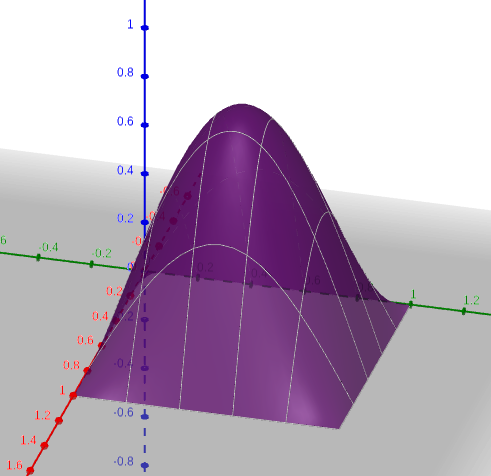
\includegraphics[width=0.75\linewidth]{Figures/sinsinEgz.png}
	\caption{Izrađeno u geogebri}
  \label{sinsinEgz}
\end{figure}

\newpage
Za elemente reda veličine $0.01$ (preciznost) moja C++ implementacija daje sljedeći 
rezultat \ref{numerSinSin001}.
\begin{figure}[H]
	\centering
  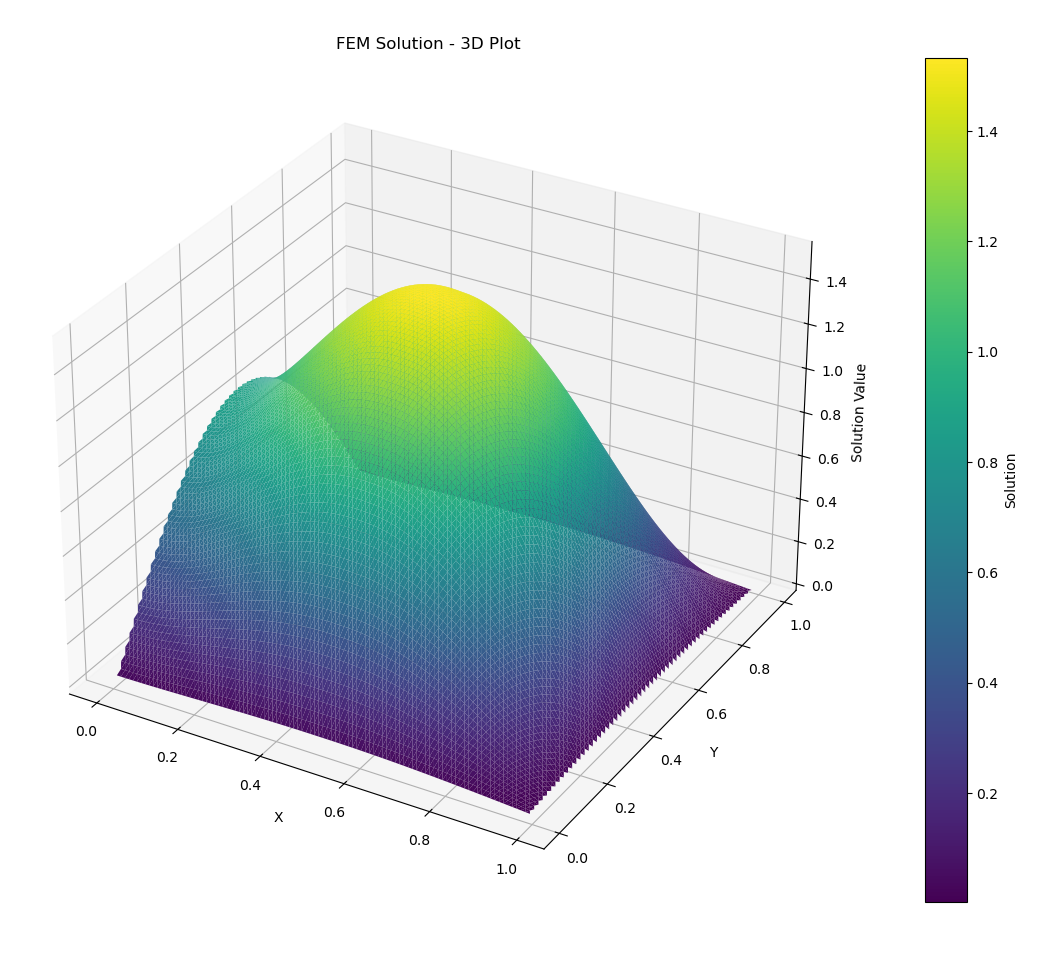
\includegraphics[width=1.2\linewidth]{Figures/numersinsin001.png}
	\caption{preciznost od $0.01$}
  \label{numerSinSin001}
\end{figure}
Vrlo se lako uoče nepravilnosti na pravcu $x=0$, 
kao i nešto veći maksimum ($1.4 > 1$)
\newpage
Dodatnim usitnjavanjem mesha (red veličine $0.0025$)
dobije se sljedeće:
\begin{figure}[H]
	\centering
	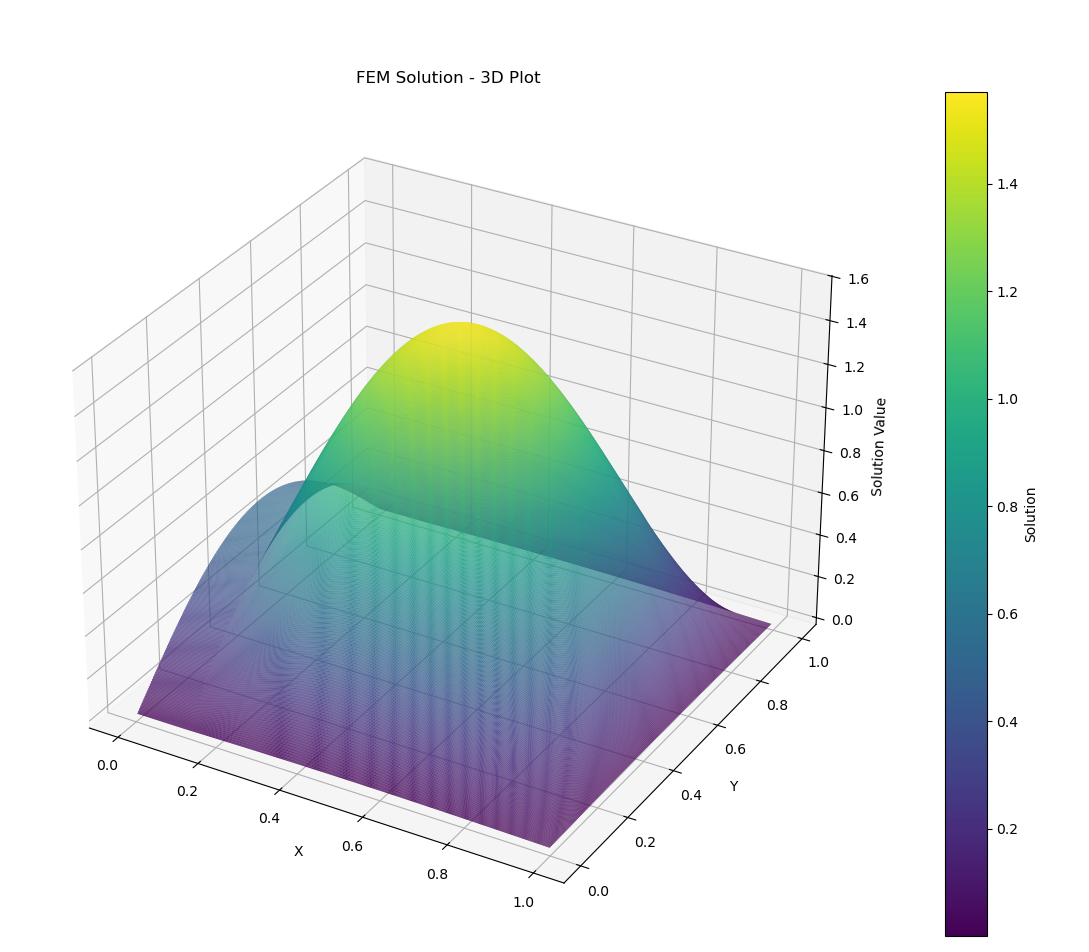
\includegraphics[width=1.2\linewidth]{Figures/numersinsin00025.png}
	\caption{preciznost od $0.00025$}
  \label{numerSinSin00025}
\end{figure}
Primijećujem kako se podignuti dio aproksimacije spustio dolje.
Nažalost, ovo nije moguće raditi u nedogled zbog potrebne 
računalne moći. Naime, usitnjavanjem mesha dolazi do više čvorova, a 
svaki čvor odgovara novoj nepoznanici koju treba riješiti u sustavu. 
S preciznošću mesha od $0.00025$ broj nepoznanica u linearnom sustavu 
iznosi redu veličine oko $10^8$, što bi moralo biti dovoljno za ovu 
 konkretnu primjenu.
\newpage
Raznim eksperimentiranjem i obzervacijama zaključio sam da je problem
u meshu. Naime, moje prve implementacije u pythonu koje su bile izrađene isključivo 
za pravokutne domene odnosno koriste mesh 
koji je bolje prilagođen obliku pravokutnika daju sljedeći rezultat:

\begin{figure}[H]
	\centering
	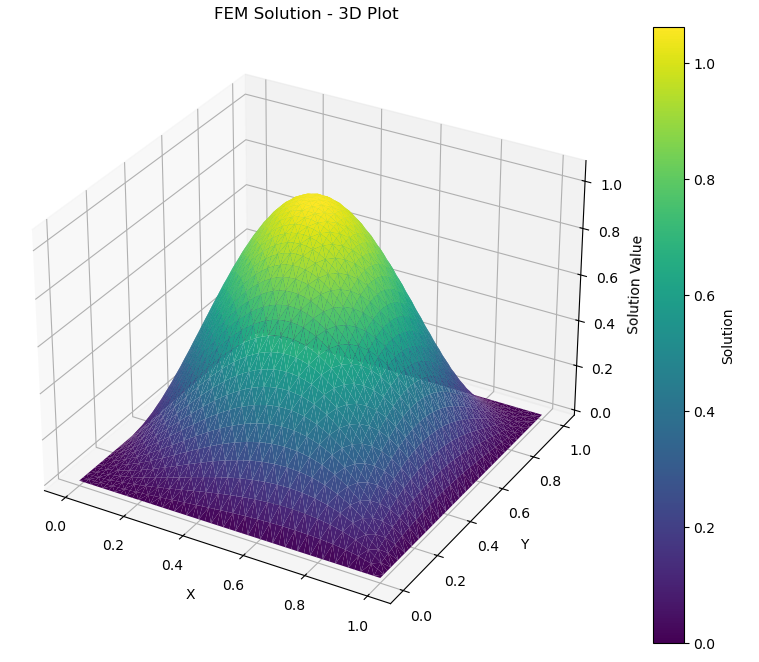
\includegraphics[width=1.15\linewidth]{Figures/numersinsin.png}
	\caption{}
  \label{numerSinSin}
\end{figure}
Ovo je očito dosta dobra aproksimacija.
\newpage
Ako usporedimo mesheve koji se koriste u ovim implementacijama,
problem postaje jasniji.

\begin{figure}[H]
  \centering
  \begin{subfigure}[b]{0.35\linewidth}
    \centering
    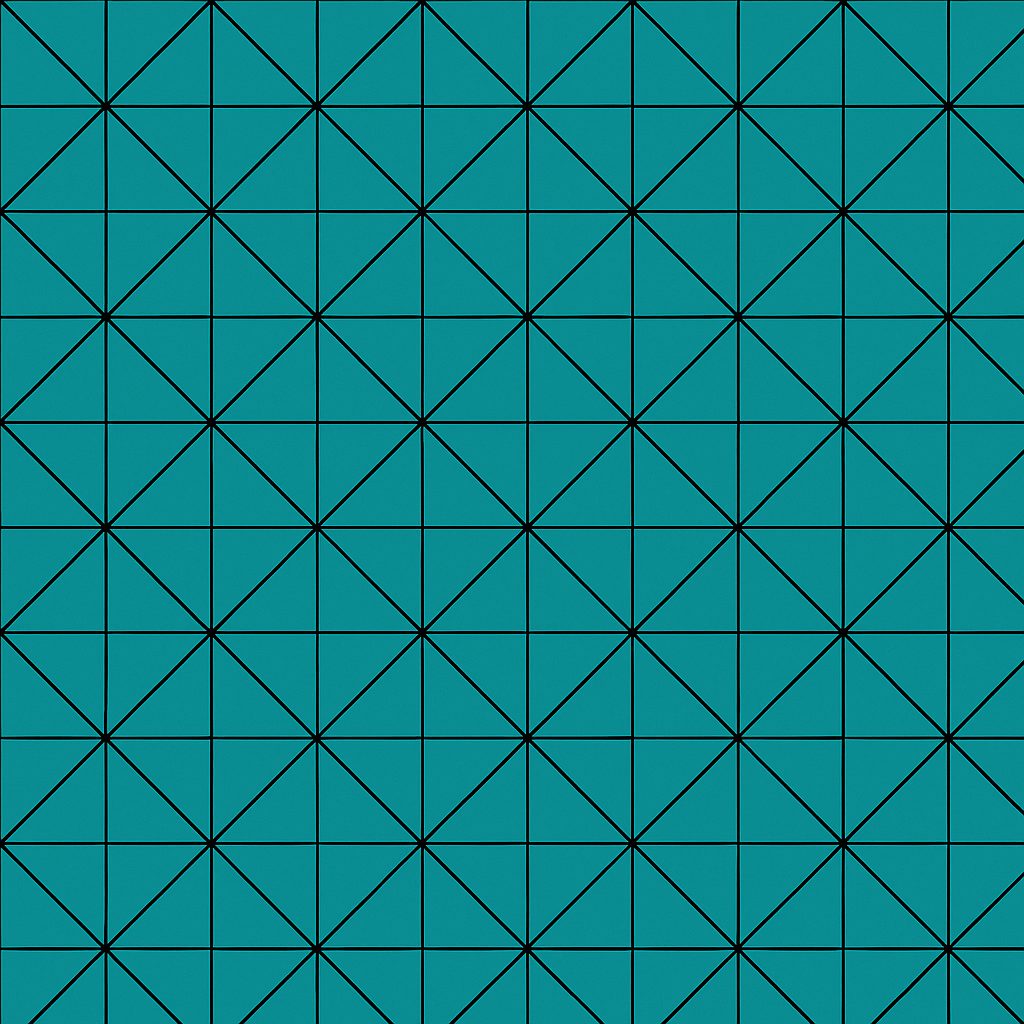
\includegraphics[width=\linewidth]{Figures/2Dmesh.png}
    \caption{Mesh prilagođeniji pravokutniku}
  \end{subfigure}
  \hfill
  \begin{subfigure}[b]{0.35\linewidth}
    \centering
    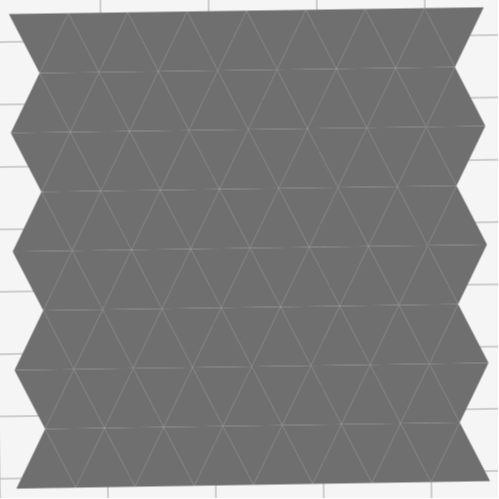
\includegraphics[width=\linewidth]{Figures/hexmesh-modified.png}
    \caption{Mesh koji daje lošije rezultate}
  \end{subfigure}
\end{figure}
Isprekinuti dio lošijeg mesha je upravo onaj dio na 
kojem se aproksimacija čudno ponaša. 
\\
Možemo pokušati riješiti pokuju PDJ i na drugačijim domenama.
\begin{equation}
  \Delta u =- 2(x +y),\, 0 \leq x, \, 0 \leq y, \, x + y \leq 1 
  \, u |_{ \partial \Omega} = 0
\end{equation}
Egzaktno rješenje glasi $u(x,y) = xy(1- x - y)$, također 
dajem i grafički prikaz \ref{xy1xy}
\begin{figure}[H]
	\centering
	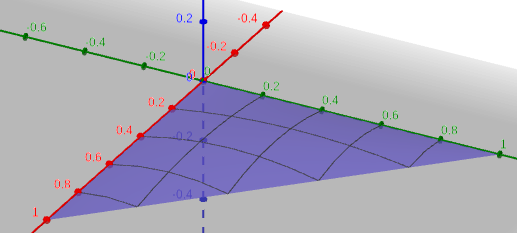
\includegraphics[width=0.8\linewidth]{Figures/xy1xy.png}
	\caption{Izrađeno u geogebri}
  \label{xy1xy}
\end{figure}
\newpage
Numeričko rješenje će se opet ponašati loše na pravcu $x=0$.

\begin{figure}[H]
	\centering
	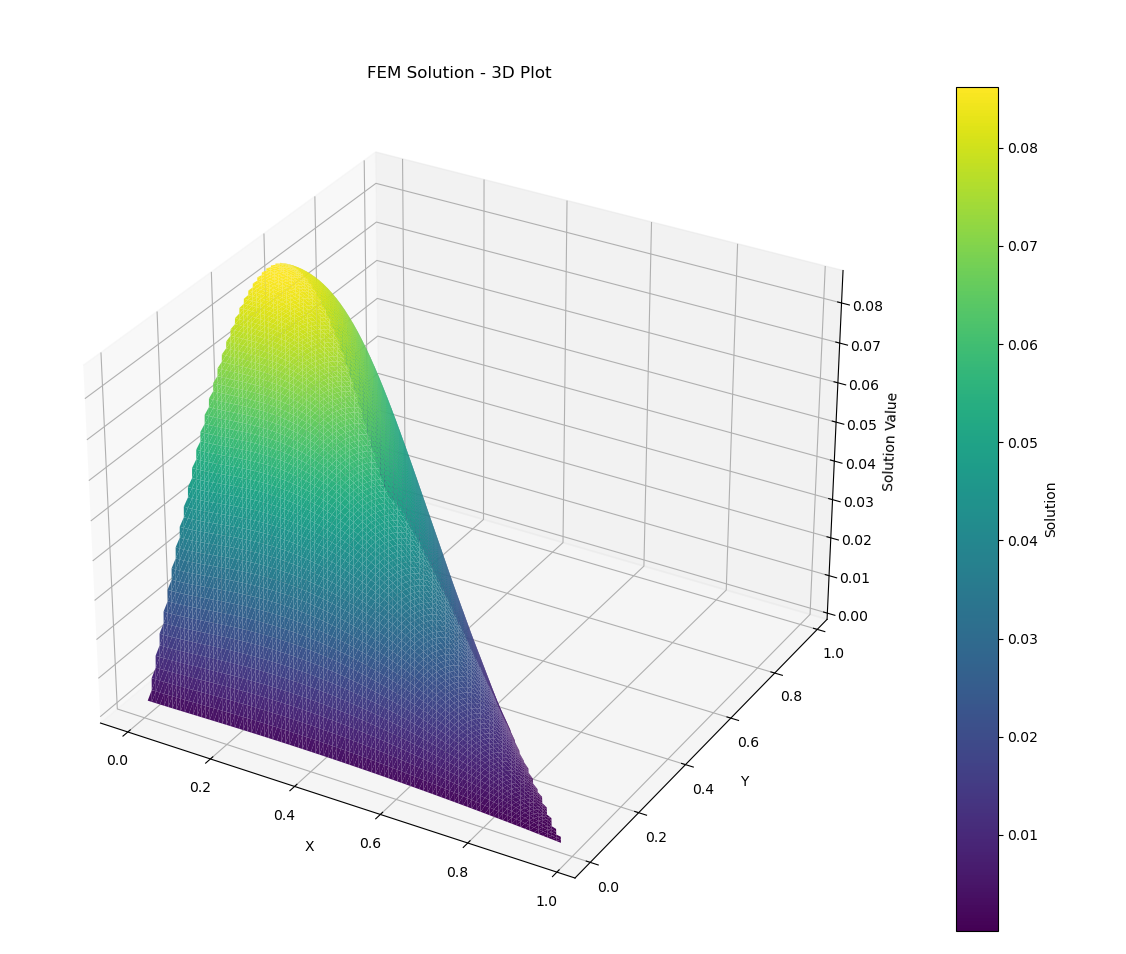
\includegraphics[width=1.2\linewidth]{Figures/numerxy1xy.png}
	\caption{preciznost od $0.01$}
  \label{}
\end{figure}
Ovaj problem može biti jedino riješen implementacijom 
kvalitetnijih generatora mesha. Moguće je također dodati i 
mogućnost unosa mesha koji su generirani od strane posebnih
alata poput Blendera, ali to nije bio cilj ovog rada. 
Cilj je bio da se mesh zadaje preko implicitnih funkcija,
a taj je problem, kako je već opisano u poglavlju o
meshevima izvan raspona ovog rada.
\newpage

%--- ZAKLJUČAK / CONCLUSION ----------------------------------------------------
\chapter{Zaključak}
Rezultatima je pokazano da je osim gustoće samog mesha,
izuzetno bitna i njegova struktura. Na primjeru jednadžbe 
potencijala s Dirichletovim uvjetima i pravokutnom domenom 
je viđeno da mesh, koji je bolje prilagođen pravokutnoj domeni, 
daje puno bolje rezultate nego onaj koji ima "cik cak" uzorak 
uz neke rubove.
\\
Analiza kroz više testnih primjera pokazala je da je ključni izazov konstrukcija 
prikladnog mesha koji može dovoljno dobro aproksimirati domenu,
a istovremeno biti računalno učinkovit.
Iako je moguće unaprijediti rezultate korištenjem
sofisticiranijih alata za generiranje mesha (npr. Blender),
fokus ovog rada bio je na izradi jednostavnog sučelja koje 
se služi implicitnom definicijom domene, slično kako bi 
ju netko definirao kada bi riješavao PDJ na papiru.
\\ 
Budući rad bi se mogao fokusirati više na izradu samog mesha
s ciljem da se ostvare bolje aproksimacije. To bi se moglo 
postići tako da se obrati puno veća pažnja na sam rub mesha 
pri smišljanju heuristike za njegovo generiranje
jer se on iz dobivenih rezultata čini važnijim. 
Također valja spomenuti i implementaciju adaptivnosti mesha 
što je metoda u kojoj se na svakom elementu procjenjuje greška 
na temelju koje se odlučuje treba li se mesh usitniti na 
dijelovima gdje je ta procijena veća.

\label{pog:zakljucak}



%--- LITERATURA / REFERENCES ---------------------------------------------------

% Literatura se automatski generira iz zadane .bib datoteke / References are automatically generated from the supplied .bib file
% Upiši ime BibTeX datoteke bez .bib nastavka / Enter the name of the BibTeX file without .bib extension
\bibliography{literatura}



%--- SAŽETAK / ABSTRACT --------------------------------------------------------

% Sažetak na hrvatskom
\begin{sazetak}
Galjorkinova metoda konačnih elemenata se često koristi
u numeričkom rješavanju (parcijalnih) diferencijalnih
jednadžbi te time ima veliki značaj u modeliranju i
rješavanju inženjerskih problema. Njezina implementacija
se bazira na raznim metodama iz numeričke matematike kao što
su rješavanje linearnih sustava i numeričko integriranje.
Složenost implementacije proizlazi i iz parcitiranja domene
na kojoj se problem rješava, a dodatna složenost je u optimizaciji
pri čemu se može koristiti višedretveno programiranje.
U ovom radu je implementirana Galjorkinova metoda te su
analizirate njene performanse na konkretnim primjerima.
\end{sazetak}

\begin{kljucnerijeci}
  diferencijalna jednadžba, parcijalna derivacija, jednadžba potencijala, FEM
\end{kljucnerijeci}


% Abstract in English
\begin{abstract}
The Galerkin finite element method is frequently
used in the numerical solution of (partial) differential
equations and thus plays an important role in modeling
and solving engineering problems.
Its implementation relies on various methods from numerical mathematics,
such as solving linear systems and numerical integration.
The complexity of the implementation also arises from the partitioning
of the domain on which the problem is solved, with additional
complexity in optimization, where multithreaded programming can be used.
In this paper, the Galerkin method was implemented and its
performance was analyzed on concrete examples.
\end{abstract}

\begin{keywords}
  differential equation, partial derivative, potential equation, FEM
\end{keywords}


%--- PRIVITCI / APPENDIX -------------------------------------------------------

% Sva poglavlje koja slijede će biti označena slovom i riječi privitak / All following chapters will be denoted with an appendix and a letter
\backmatter

\chapter{The Code}
\begin{itemize}
 \item \href{https://github.com/hrvojerados/CppFEM-Library}{C++ implementacija}

 \item \href{https://github.com/hrvojerados/FiniteElementMethods}{Python implementacija}
\end{itemize}
\end{document}
